\chapter{Les variables}

Programmer, c'est avant tout donner des ordres à
notre ordinateur afin qu'il réalise ce que l'on souhaite. Ces ordres
vont permettre à notre ordinateur de manipuler de l'information sous
différentes formes (nombres, textes, vidéos, etc). À ce stade, nous
savons que ces ordres, ces instructions sont exécutées par notre
processeur. Cependant, nous ne savons toujours pas comment donner des
ordres, ni comment manipuler de l'information.

Ce chapitre vous expliquera comment manipuler les types de données les
plus simples du langage C, les nombres et les lettres (ou caractères),
grâce à ce qu'on appelle des \textbf{variables}. Après celui-ci, vous
pourrez ainsi profiter de votre ordinateur comme s'il s'agissait d'une
grosse calculatrice. Néanmoins, rassurez-vous, le niveau en maths de ce
chapitre sera assez faible : si vous savez compter, vous pourrez le
comprendre facilement !

Cela peut paraitre un peu bête et pas très intéressant, mais il faut
bien commencer par les bases. Manipuler du texte ou de la vidéo est
complexe et nécessite en plus de savoir comment manipuler des nombres.
\emph{Eh} oui ! Comme vous allez le voir, tout est nombre pour notre
ordinateur, même le texte et la vidéo.

\section{Qu’est-ce qu’une variable ?}

Pour comprendre ce qu'est une variable et comment manipuler celles-ci,
il faut commencer par comprendre comment notre ordinateur fait pour
stocker des données. En théorie, un ordinateur est capable de stocker
tout type d'information. Mais comment est-il possible de réaliser un
tel miracle alors qu'il ne s'agit finalement que d'un amas de circuits
électriques ?

\subsection{Codage des informations}\label{codage-des-informations}

Peut-être avez-vous déjà entendu le proverbe suivant : « si le seul
outil que vous avez est un marteau, vous verrez tout problème comme un
clou » (Abraham Maslow). \emph{Hé} bien, l'idée est un peu la même
pour un ordinateur : ce dernier ne sachant utiliser que des nombres,
il voit toute information comme une suite de nombres.

L'astuce consiste à transformer une information en nombre pour que
l'ordinateur puisse la traiter, autrement dit la \textbf{numériser}.
Différentes techniques sont possibles pour atteindre cet objectif, une
des plus simples étant une table de correspondance, par exemple entre
un nombre et un caractère.

\begin{table}[ht!]
\centering
\begin{tabular}{|l|l|}\hline
\rowcolor{gris-tab-entete}Caractère & Nombre \\ \hline
\rowcolor{gris-clair-tab}A	  & 1      \\ \hline 
B	  & 2      \\ \hline
\rowcolor{gris-clair-tab}C  	  & 3      \\ \hline
\end{tabular}
\end{table}

\subsection{Binaire}\label{binaire}

Cependant, comme si cela ne suffisait pas, un ordinateur ne compte pas
comme nous : il compte en base deux (l'andouille !).

\begin{questionbox}
En base deux ?
\end{questionbox}

La base correspond au nombre de chiffres disponibles pour représenter
un nombre. En base 10, nous disposons de dix chiffres : zéro, un,
deux, trois, quatre, cinq, six, sept, huit et neuf. En base deux, nous
en avons donc\ldots{} deux : zéro et un. Pour ce qui est de compter,
c'est du pareil au même : nous commençons par épuiser les unités : 0,
1 ; puis nous passons aux dizaines : 10, 11 ; puis aux centaines :
100, 101, 110, 111 ; et ainsi de suite. Ci-dessous un petit tableau de
correspondance entre la base deux et la base dix.

\begin{table}[ht!]
\centering
\begin{tabular}{|l|l|}\hline
\rowcolor{gris-tab-entete}\textbf{Base deux} & \textbf{Base dix}\tabularnewline\hline
\rowcolor{gris-clair-tab}0 & 0\tabularnewline\hline
1 & 1\tabularnewline\hline
\rowcolor{gris-clair-tab}10 & 2\tabularnewline\hline
11 & 3\tabularnewline\hline
\rowcolor{gris-clair-tab}100 & 4\tabularnewline\hline
101 & 5\tabularnewline\hline
\rowcolor{gris-clair-tab}110 & 6\tabularnewline\hline
111 & 7\tabularnewline\hline
\rowcolor{gris-clair-tab}1000 & 8\tabularnewline\hline
1001 & 9\tabularnewline\hline
\rowcolor{gris-clair-tab}1010 & 10\tabularnewline\hline
\end{tabular}
\caption{Correspondance base deux-base dix}
\end{table}

Un chiffre binaire (un zéro ou un un) est appelé un \emph{bit} en
anglais. Il s'agit de la contraction de l'expression « \emph{binary
  digit} ». Nous l'emploierons assez souvent dans la suite de ce cours
par souci d'économie.

\begin{questionbox}
 Mais pourquoi utiliser la base deux et non la base dix ?
\end{questionbox}



Parce que les données circulent sous forme de courants
électriques. Or, la tension de ceux-ci n'étant pas toujours stable, il
est difficile de réaliser un système fiable sachant détecter dix
valeurs différentes. Par contre, c'est parfaitement possible avec deux
valeurs : il y a du courant ou il n'y en a pas.

\section{La mémoire}\label{la-memoire}

Nous savons à présent que notre ordinateur ne sait employer que des
nombres représentés en base deux.

\begin{questionbox}
 Mais comment stocker tout ce fatras de nombres ?
\end{questionbox}


\emph{Hé} bien, les \emph{bits} sont stockés dans un composant
électronique particulier de l'ordinateur : la \textbf{mémoire}. Enfin,
nous disons « \textbf{la} mémoire », mais il y en a en fait plusieurs.

\begin{questionbox}
 Mais pourquoi plusieurs mémoires et pas une seule ?
\end{questionbox}


Le fait est qu'il est actuellement impossible de créer des mémoires
qui soient à la fois rapides et capables de contenir beaucoup de
données.  Nous ne pouvons donc utiliser une seule grosse mémoire
capable de stocker toutes les données dont nous avons besoin. Ce
problème s'est posé dès les débuts de l'informatique, comme en
témoigne cette citation des années 1940, provenant des concepteurs
d'un des tout premiers ordinateurs.

\begin{quote}
  Idéalement, nous désirerions une mémoire d'une capacité indéfiniment
  large telle que n'importe quelle donnée soit immédiatement
  accessible.  Nous sommes forcés de reconnaître la possibilité de la
  construction d'une hiérarchie de mémoire, chacune ayant une capacité
  plus importante que la précédente, mais accessible moins
  rapidement. Source: Burks, Goldstine, et Von Neumann
\end{quote}

Mais les chercheurs et ingénieurs du début de l'informatique ont
trouvé une solution : segmenter la mémoire de l'ordinateur en
plusieurs sous-mémoires, de taille et de vitesse différentes,
utilisées chacune suivant les besoins. Nous aurons donc des mémoires
pouvant contenir peu de données et rapides, à côté de mémoires plus
importantes et plus lentes.

Nous vous avons dit que l'ordinateur utilisait plusieurs
mémoires. Trois d'entre elles méritent à notre sens votre attention :

\begin{itemize}
\item
  les registres ;
\item
  la mémoire vive (ou RAM en anglais) ;
\item
  le disque dur.
\end{itemize}

*{[}RAM{]}: Random Access Memory

Les \textbf{registres} sont des mémoires intégrées dans le processeur,
utilisées pour stocker des données temporaires. Elles sont très
rapides, mais ne peuvent contenir que des données très simples, comme
des nombres.

La \textbf{mémoire vive} est une mémoire un peu plus grosse, mais plus
lente que les registres. Elle peut contenir pas mal de données et est
généralement utilisée pour stocker les programmes en court d'exécution
ainsi que les données qu'ils manipulent.

Ces deux mémoires (les registres et la mémoire vive) ont tout de même
un léger défaut : elles perdent leur contenu quand elles ne sont plus
alimentées\ldots{} Autant dire que ce n'est pas le meilleur endroit
pour stocker un système d'exploitation ou des fichiers
personnels. Ceci est le rôle du \textbf{disque dur}, une mémoire avec
une capacité très importante, mais très lente qui a toutefois
l'avantage d'assurer la persistance des données.

En C, la mémoire la plus manipulée par le programmeur est la mémoire
vive. Aussi, nous allons nous y intéresser d'un peu plus près dans ce
qui suit.

\subsubsection{Bits, multiplets et octets}\label{bits-multiplets-et-octets}

Dans la mémoire vive, les \emph{bits} sont regroupés en « paquets » de
quantité fixe : des « \textbf{cases mémoires} », aussi appelées
\textbf{multiplets} (ou \emph{bytes} en anglais). À quelques exceptions
près, les mémoires utilisent des multiplets de huit \emph{bits}, aussi
appelés \textbf{octet}. Un octet peut stocker 256 informations
différentes (vous pouvez faire le calcul vous-même : combien vaut
11111111 en base deux ? :p ). Pour stocker plus d'informations, il sera
nécessaire d'utiliser plusieurs octets.


\subsection{Adresse mémoire}\label{adresse-muxe9moire}

Néanmoins, il est bien beau de stocker des données en mémoire, encore
faut-il pouvoir remettre la main dessus.

Dans cette optique, chaque octet de la mémoire vive se voit attribuer
un nombre unique, \textbf{une adresse}, qui va permettre de le
sélectionner et de l'identifier parmi tous les autres. Imaginez la
mémoire vive de l'ordinateur comme une immense armoire, qui
contiendrait beaucoup de tiroirs (les cases mémoires) pouvant chacun
contenir un octet. Chaque tiroir se voit attribuer un numéro pour le
reconnaitre parmi tous les autres. Nous pourrions ainsi demander quel
est le contenu du tiroir numéro 27. Pour la mémoire, c'est
pareil. Chaque case mémoire a un numéro : son adresse.

\begin{table}[ht!]
\centering
\rowcolors{1}{gris-clair-tab}{}
\begin{tabular}{|l|l|}
\hline
\rowcolor{gris-tab-entete}\textbf{Adresse} & \textbf{Contenu mémoire}\tabularnewline\hline
0 & 11101010\tabularnewline\hline
1 & 01111111\tabularnewline\hline
2 & 00000000\tabularnewline\hline
3 & 01010101\tabularnewline\hline
4 & 10101010\tabularnewline\hline
5 & 00000000\tabularnewline\hline
\end{tabular}
\caption{Adresse mémoire}
\end{table}

En fait, vous pouvez comparer une adresse à un numéro de téléphone :
chacun de vos correspondants a un numéro de téléphone et vous savez
que pour appeler telle personne, vous devez composer tel numéro. Les
adresses mémoires fonctionnent exactement de la même façon !

\begin{figure}[ht!]
\centering
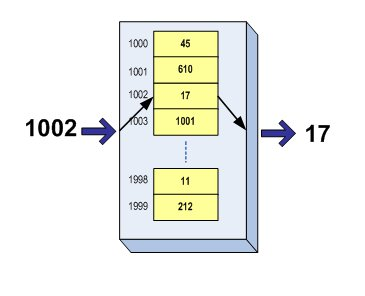
\includegraphics[scale=0.6]{images/adresse_memoire.jpg}
\caption{Exemple : on demande à notre mémoire de sélectionner la case
mémoire d'adresse 1002 et on récupère son contenu (ici, 17).}
\end{figure}

\begin{infobox}
  Plus généralement, toutes les mémoires disposent d'un mécanisme
  similaire pour retrouver les données.  Aussi, vous entendrez souvent
  le terme de \textbf{référence} qui désigne un moyen (comme une
  adresse) permettant de localiser une donnée. Il s'agit simplement
  d'une notion plus générale.
\end{infobox}

\subsection{Les variables}
\label{les-variables}

Tout cela est bien sympathique, mais manipuler explicitement des
références (des adresses si vous préférez) est un vrai calvaire, de
même que de s'évertuer à calculer en base deux. Heureusement pour
nous, les langages de programmation (et notamment le C), se chargent
d'effectuer les conversions pour nous et remplacent les références par
des variables.

Une variable correspondra à une portion de mémoire, appelée
\textbf{objet}, à laquelle nous donnerons un nom. Ce nom permettra
d'identifier notre variable, tout comme une référence permet
d'identifier une portion de mémoire parmi toutes les autres. Nous
allons ainsi pouvoir nommer les données que nous manipulons, chacun de
ces noms étant remplacés lors de la compilation par une référence (le
plus souvent une adresse).

\section{Déclarer une variable}
\label{declarer-une-variable}

Entrons maintenant dans le vif du sujet en apprenant à déclarer nos
variables. Tout d'abord, sachez qu'une variable est constituée de deux
éléments obligatoires :

\begin{itemize}
\item
  un \textbf{type} ;
\item
  un \textbf{identificateur} qui est en gros le « nom » de la variable.
\end{itemize}

Le type d'une variable permet d'indiquer ce qui y sera stocké, par
exemple : un caractère, un nombre entier, un nombre à virgule (ou
nombre \textbf{flottant}), etc. Pour préciser le type d'une variable,
il est nécessaire d'utiliser un mot-clé spécifique (il y en a donc un
pour chaque type).

Une fois que nous avons décidé du nom et du type de notre variable,
nous pouvons la créer (on dit aussi la déclarer) comme suit.

\begin{C}
type identificateur;
\end{C}

En clair, il suffit de placer un mot-clé indiquant le type de la
variable et de placer le nom qu'on lui a choisi immédiatement après.

\begin{attentionbox}
  Faites bien attention au point-virgule à la fin !
\end{attentionbox}

\subsection{Les types}
\label{les-types}

Comme dit précédemment, un type permet d'indiquer au compilateur quel
genre de données nous souhaitons stocker. Ce type va permettre de
préciser :

\begin{itemize}
\item
  toutes les valeurs que peut prendre la variable ;
\item les opérations qu'il est possible d'effectuer avec (il n'est par
  exemple pas possible de réaliser une division entière avec un nombre
  flottant, nous y reviendrons).
\end{itemize}

Définir le type d'une variable permet donc de préciser son contenu
potentiel et ce que nous pouvons faire avec. Le langage C fournit
sept\footnote{\footnotesize{Depuis la norme C99, un type entier
    supplémentaire a été ajouté : le type \mybox{long\ long\ int}. Ses
    bornes garanties par la norme sont comprises entre -9 223 372 036
    854 775 807 et 9 223 372 036 854 775 807 s'il est signé et entre 0
    et 18 446 744 073 709 551 615 s'il est non signé.}} types de base.

\begin{table}[ht!]
\centering
\rowcolors{1}{gris-clair-tab}{}
\begin{tabular}{|l|l|}\hline
\rowcolor{gris-tab-entete}\textbf{Type} & \textbf{Sert à stocker}\tabularnewline\hline
\textbf{char} & un caractère ou un entier\tabularnewline\hline
\textbf{short int} & un entier\tabularnewline\hline
\textbf{int} & un entier\tabularnewline\hline
\textbf{long int} & un entier\tabularnewline\hline
\textbf{float} & un flottant\tabularnewline\hline
\textbf{double} & un flottant\tabularnewline\hline
\textbf{long double} & un flottant\tabularnewline\hline
\end{tabular}
\caption{Les 7 types de base}
\end{table}

Les types \mybox{short\ int}, \mybox{int} et \mybox{long\ int} servent
tous à stocker des nombres entiers qui peuvent prendre des valeurs
positives, négatives, ou nulles. On dit qu'il s'agit de types signés
(car il peut comporter un signe). Pour ces trois types, il existe un
type équivalent dit \textbf{non signé}. Un type entier non signé est
un type entier qui n'accepte que des valeurs positives ou nulles : il
ne peut pas stocker de valeurs négatives. Pour déclarer des variables
d'un type non signé, il vous suffit de faire précéder le nom du type
entier du mot-clé \mybox{unsigned}.

Le type \mybox{char} peut lui aussi servir à stocker des nombres. Il
sert surtout au stockage de caractères, mais ces derniers étant
stockés dans l'ordinateur sous forme de nombres, il est possible de
stocker des nombres dans un \mybox{char}. Le seul problème, c'est que
ce type peut être signé ou non signé de base suivant les
compilateurs. Pour éviter les ennuis, spécifiez ce que vous souhaitez
lors de la déclaration : non signé (\mybox{unsigned\ char}) ou signé
(\mybox{signed\ char}).

{\begin{infobox} En cas de manque d'information concernant le type
    lors d'une déclaration, c'est le type \mybox{int} qui sera
    utilisé. Ainsi, \mybox{long} et \mybox{short} sont respectivement
    des raccourcis pour \mybox{long\ int} et \mybox{short\ int}. De
    même, le mot-clé \mybox{unsigned} seul signifie \mybox{unsigned\
      int}.
\end{infobox}

\subsubsection{Capacité d'un type}
\label{capacite-dun-type}

Tous les types stockant des nombres ont des bornes, c'est-à-dire une
limite aux valeurs qu'ils peuvent stocker. En effet, le nombre de
multiplets occupés par une variable est limité suivant son type. En
conséquence, il n'est pas possible de mettre tous les nombres
possibles dans une variable de type \mybox{int}, \mybox{float}, ou
\mybox{double}. Il y aura \emph{toujours} une valeur minimale et une
valeur maximale. Ces limites sont les suivantes.

\begin{table}[ht!]
\centering
\rowcolors{1}{gris-clair-tab}{}
\begin{tabular}{|l|l|l|}\hline
\rowcolor{gris-tab-entete}\textbf{Type} & \textbf{Minimum} & \textbf{Maximum}\tabularnewline\hline
\textbf{signed char} & -127 & 127\tabularnewline\hline
\textbf{unsigned char} & 0 & 255\tabularnewline\hline
\textbf{short} & -32 767 & 32 767\tabularnewline\hline
\textbf{unsigned short} & 0 & 65 535\tabularnewline\hline
\textbf{int} & -32 767 & 32 767\tabularnewline\hline
\textbf{unsigned int} & 0 & 65 535\tabularnewline\hline
\textbf{long} & -2 147 483 647 & 2 147 483 647\tabularnewline\hline
\textbf{unsigned long} & 0 & 4 294 967 295\tabularnewline\hline
\textbf{float} & -1 × 10\textsuperscript{37} & 1 × 10\textsuperscript{37}\tabularnewline\hline
\textbf{double} & -1 × 10\textsuperscript{37} & 1 × 10\textsuperscript{37}\tabularnewline\hline
\textbf{long double} & -1 × 10\textsuperscript{37} & 1 × 10\textsuperscript{37}\tabularnewline\hline
\end{tabular}
\caption{Les limites des types}
\end{table}

Si vous regardez bien ce tableau, vous remarquez que certains types ont
des bornes identiques. En vérité, les valeurs présentées ci-dessus sont
les minimums garantis par la norme\footnote{\footnotesize{Programming Language C,
  X3J11/88-090, § 2.2.4.2, Numerical limits}}

\subsubsection{Taille d'un type}
\label{taille-dun-type}

Peut-être vous êtes vous demandés pourquoi il existe autant de types
différents. La réponse est toute simple : la taille des mémoires était
très limitée à l'époque où le langage C a été créé. En effet, le
\href{https://upload.wikimedia.org/wikipedia/commons/c/c4/80_early_pcp_2.jpg}{PDP-11}
sur lequel le C a été conçu ne possédait que 24Ko de mémoire (pour
comparaison, une calculatrice TI-Nspire possède 100Mo de mémoire, soit
environ 4000 fois plus). Il fallait donc l'économiser au maximum en
choisissant le type le plus petit possible. Cette taille dépend des
machines, mais de manière générale, vous pouvez retenir les deux suites
d'inégalités suivantes : \mybox{char} ≤ \mybox{short} ≤ \mybox{int} ≤
\mybox{long} et \mybox{float} ≤ \mybox{double} ≤
\mybox{long\ double}.

Aujourd'hui ce n'est plus un problème, il n'est pas nécessaire de se
casser la tête sur quel type choisir (excepté si vous voulez programmer
pour de petits appareils où la mémoire est plus petite). En pratique,
nous utiliserons surtout \mybox{char} pour les caractères, \mybox{int}
ou \mybox{long} pour les entiers et \mybox{double} pour les flottants.

\subsection{Les identificateurs}
\label{les-identificateurs}

Maintenant que nous avons vu les types, parlons des identificateurs.
Comme dit précédemment, un identificateur est un nom donné à une
variable pour la différencier de toutes les autres. Et ce nom, c'est
au programmeur de le choisir. Cependant, il y a quelques limitations à
ce choix.

\begin{itemize}
\item seuls les 26 lettres de l'alphabet latin (majuscules ou
  minuscules), le trait de soulignement « \_ » (\emph{underscore} en
  anglais) et les chiffres sont acceptés. Pas d'accents, pas de
  ponctuation ni d'espaces ;
\item
  un identificateur ne peut pas commencer par un chiffre ;
\item
  les mots-clés ne peuvent pas servir à identifier une variable ; il
  s'agit de :
\end{itemize}

\begin{C}
auto     double  int       struct
break    else    long      switch
case     enum    register  typedef
char     extern  return    union
const    float   short     unsigned
continue for     signed    void
default  goto    sizeof    volatile
do       if      static    while
\end{C}

\begin{itemize}
\item deux variables ne peuvent avoir le même identificateur (le même
  nom).  Il y a parfois quelques exceptions, mais cela n'est pas pour
  tout de suite ;
\item
  les identificateurs peuvent être aussi longs que l'on désire,
  toutefois le compilateur ne tiendra compte que des 31 premiers
  caractères.
\end{itemize}

Voici quelques exemples pour bien comprendre.

\begin{table}[ht!]
\centering
\rowcolors{1}{gris-clair-tab}{}
\begin{tabular}{|l|l|l|}\hline
\rowcolor{gris-tab-entete}\textbf{Identificateur correct} & \textbf{Identificateur incorrect} & \textbf{Raison}\tabularnewline\hline
variable & Nom de variable & Espaces interdits\tabularnewline\hline
nombre\_de\_vie & 1nombre\_de\_vie & Commence par un chiffre\tabularnewline\hline
test & test! & Caractère « ! » interdit\tabularnewline\hline
un\_dernier\_pour\_la\_route1 & \mybox{continue} & Mot-clé réservé par le langage\tabularnewline\hline
\end{tabular}
\caption{Les identificateurs}
\end{table}

À noter que le C fait la différence entre les majuscules et les
minuscules (on dit qu'\textbf{il respecte la casse}). Ainsi les trois
identificateurs suivants sont différents.

\begin{C}
variable
Variable
VaRiAbLe
\end{C}

\subsection{Déclaration et initialisation}
\label{declaration-et-initialisation}

Maintenant que nous connaissons toutes les bases, entrainons-nous à
déclarer quelques variables.

\begin{C}
int main(void)
}
    double taille;
    unsigned int age;
    char caractere;
    short petite_valeur;

    return 0;
}
\end{C}

Il est possible de déclarer plusieurs variables \textbf{de même type}
sur une même ligne, en séparant leurs noms par une virgule.

\begin{C}
int age, taille, nombre;
\end{C}

Ceci permet de regrouper les déclarations suivant les rapports que les
variables ont entre elles.

\begin{C}
int annee, mois, jour;
int age, taille;
int x, y, z;
\end{C}

\subsubsection{Initialisation}
\label{initialisation}

En plus de déclarer une variable, il est possible de
\textbf{l'initialiser}, c'est-à-dire de lui attribuer une valeur. La
syntaxe est la suivante.

\begin{C}
type identificateur = valeur;
\end{C}

Ou comme ceci s'il s'agit d'un caractère.

\begin{C}
char identificateur = 'lettre';
\end{C}

Quelques exemples d'initialisations de variables.

\begin{C}
unsigned int age =25;
short petite_valeur =1;
const long abc =314159265;
char caractere = 'h';
\end{C}

\begin{infobox}
  Notez qu'une déclaration comporte le mot-clé \mybox{const}. Celui-ci
  permet de préciser qu'une variable ne pourra pas être modifiée par
  la suite. Ceci peut être utile pour stocker une valeur qui ne
  changera jamais (comme la constante \(\pi\) qui vaut toujours
  3,14159265).
\end{infobox}

\begin{attentionbox}
  Les déclarations doivent toujours se situer en début de bloc,
  c'est-à-dire juste après une accolade ouvrante.
\end{attentionbox}


\subsubsection{Initialisation des nombres flottants}
\label{initialisation-des-nombres-flottants}

\subsubsection*{En notation simple}

Petite précision concernant la manière d'initialiser une variable de
type flottant : celles-ci étant faites pour contenir des nombres à
virgule, à l'initialisation, il est nécessaire de placer cette «
virgule ». Toutefois, cette dernière est représentée par un point.

\begin{C}
const double pi = 3.14;
\end{C}

Ceci vient du fait que le C est une invention américaine et que les
anglophones utilisent le point à la place de la virgule.

Notez qu'il est important de bien placer ce point, \emph{même si vous
  voulez stocker un nombre entier}. Par exemple, vous ne devez pas
écrire \mybox{double a = 5} mais \mybox{double a = 5.} (certains
préfèrent \mybox{double a = 5.0}, cela revient au même). Si vous ne le
faites pas, vous risquez d'avoir quelques problèmes.

\subsubsection*{En notation scientifique}

Par ailleurs, sachez qu'il est également possible de représenter un
nombre flottant à l'aide de la notation scientifique, c'est-à-dire
sous la forme d'un nombre décimal et d'une puissance de dix. Cela se
traduit par un nombre flottant en notation simple (comme ci-dessus)
suivi de la lettre « e » ou « E » et d'un exposant \emph{entier}.

\begin{C}
double f = 1E-1; /* 1x10^-1 = 0.1 */
\end{C}

\subsection{Affectation}\label{affectation}

Nous savons donc déclarer (créer) nos variables et les initialiser
(leur donner une valeur à la création). Il ne nous reste plus qu'à
voir la dernière manipulation possible :
\textbf{l'affectation}. Celle-ci permet de modifier la valeur contenue
dans une variable pour la remplacer par une autre valeur.

Il va de soi que cette affectation n'est possible que pour les variables
qui ne sont pas déclarées avec le mot-clé \mybox{const} puisque, par
définition, de telles variables sont constantes et ne peuvent voir leur
contenu modifié.

Pour faire une affectation, il suffit d'opérer ainsi.

\begin{C}
identificateur = nouvelle_valeur;
\end{C}

Nous voyons que la syntaxe est similaire à celle d'une déclaration
avec initialisation. La seule différence, c'est que nous n'avons pas à
préciser le type. Celui-ci est en effet fixé une fois pour toute lors
de la déclaration de notre variable. Aussi, il n'est pas nécessaire de
le préciser à nouveau lors d'une affectation.

\begin{C}
age = 30;
taille = 177.5;
petite_valeur = 2
\end{C}

Notez qu'il n'y a aucune limite au nombre d'affectations, comme le
démontre l'exemple ci-dessous.

\begin{C}
petite_valeur = 2;
petite_valeur = 4;
petite_valeur = 8;
petite_valeur = 16;
petite_valeur = 8;
petite_valeur = 4;
petite_valeur = 2;
\end{C}

À chaque affectation, la variable va prendre une nouvelle valeur. Par
contre, ne mettez pas le type quand vous voulez changer la valeur,
sinon vous aurez le droit à une belle erreur du type «
\emph{redefinition of `nom\_de\_votre\_variable'} » car vous aurez
créé deux variables avec le même identificateur !

Le code suivant est donc incorrect.

\begin{C}
int age =15;
int age =20;
\end{C}

Si vous exécutez tous ces codes, vous verrez qu'ils n'affichent
toujours rien et c'est normal puisque nous n'avons pas demandé à notre
ordinateur d'afficher quoique ce soit. Nous apprendrons comment faire
au chapitre suivant.

\begin{erreurbox} Il n'y a pas de valeur par défaut en C.  Aussi, sans
  initialisation ou affectation, la valeur d'une variable est
  indéterminée ! Veillez donc à ce que vos variables aient une valeur
  connue avant de les utiliser !
\end{erreurbox}

\section{Les représentations octales et hexadécimales }

Pour terminer ce chapitre, nous vous proposons un petit aparté sur
deux représentations particulières : la représentation octale et la
représentation hexadécimale.

Nous avons déjà vu la représentation binaire au début de ce chapitre,
les représentations octale et hexadécimale obéissent au même schéma :
au lieu d'utiliser dix chiffres pour représenter un nombre, nous en
utilisons respectivement huit ou seize.

\begin{questionbox}
  Seize chiffres ?! Mais\ldots{} Je n'en connais que dix moi !
\end{questionbox}

La représentation hexadécimale est un peu déroutante de prime abord,
celle-ci ajoute six chiffres (en fait, six lettres) : a, b, c, d, e et
f. Pour vous aider, voici un tableau présentant les nombres de 1 à 16
en binaire, octal, décimal et hexadécimal.

\begin{table}[ht!]
\centering
\rowcolors{1}{gris-clair-tab}{}
\begin{tabular}{|l|l|l|l|}\hline
\rowcolor{gris-tab-entete}\textbf{Binaire} & \textbf{Octal} & \textbf{Décimal} & \textbf{Hexadécimal}\tabularnewline\hline
00001 & 1 & 1 & 1\tabularnewline\hline
00010 & 2 & 2 & 2\tabularnewline\hline
00011 & 3 & 3 & 3\tabularnewline\hline
00100 & 4 & 4 & 4\tabularnewline\hline
00101 & 5 & 5 & 5\tabularnewline\hline
00110 & 6 & 6 & 6\tabularnewline\hline
00111 & 7 & 7 & 7\tabularnewline\hline
01000 & 10 & 8 & 8\tabularnewline\hline
01100 & 14 & 12 & c\tabularnewline\hline
01101 & 15 & 13 & d\tabularnewline\hline
01110 & 16 & 14 & e\tabularnewline\hline
01111 & 17 & 15 & f\tabularnewline\hline
10000 & 20 & 16 & 10\tabularnewline\hline
\end{tabular}
\caption{Les nombres de 1 à 16 en binaire, octal, décimal et hexadécimal}
\end{table}

\begin{infobox}
  Notez que dix dans n'importe quelle base équivaut à cette base.
\end{infobox}

\begin{questionbox}
  Quel est l'intérêt de ces deux bases exactement ?
\end{questionbox}
  
L'avantage des représentations octale et hexadécimale est qu'il est
facilement possible de les convertir en binaire contrairement à la
représentation décimale. En effet, un chiffre en base huit ou en base
seize peut-être facilement traduit, respectivement, en trois ou quatre
\emph{bits}.

Prenons l'exemple du nombre 35 qui donne 43 en octal et 23 en
hexadécimal. Nous pouvons nous focaliser sur chaque chiffre un à un
pour obtenir la représentation binaire. Ainsi, du côté de la
représentation octale, 4 donne \mybox{100} et 3 \mybox{011}, ce qui
nous donne finalement \mybox{00100011}. De même, pour la
représentation hexadécimale, 2 nous donne \mybox{0010} et 3
\mybox{0011} et nous obtenons \mybox{00100011}. Il n'est pas possible
de faire pareil en décimal.

En résumé, les représentations octale et hexadécimale permettent de
représenter un nombre binaire de manière plus concise et plus lisible.

\section{Constantes octales et
hexadécimales}\label{constantes-octales-et-hexaduxe9cimales}

Il vous est possible de préciser la base d'une constante entière en
utilisant des préfixes. Ces préfixes sont \mybox{0} pour les
constantes octales et \mybox{0x} ou \mybox{0X} pour les constantes
hexadécimales.

\begin{C}
long a = 65535; /* En décimal */
int b =0777; /* En octal */
short c = 0xFF; /* En hexadécimal */
\end{C}

\begin{infobox}
  Les lettres utilisées pour la représentation hexadécimale peuvent
  être aussi bien écrites en minuscule qu'en majuscule.
\end{infobox}


\begin{questionbox}
  Il n'est pas possible d'utiliser une constante en base deux ?
\end{questionbox}

Malheureusement, non, le langage C ne permet pas d'utiliser de telles
constantes.

\hrulefill
    
Voilà, c'est la fin de ce chapitre. Nous avons vu beaucoup de choses,
n'hésitez pas à potasser pour bien assimiler tout ça. Les variables
sont vraiment la base de la programmation, aussi il nécessaire de bien
les comprendre. Rendez-vous au prochain chapitre qui sera très
intéressant : vous pourrez par exemple demander l'âge de l'utilisateur
pour ensuite l'afficher !